\chapter{Objetivos}\label{cap:2}
\lettrine{C}{uáles son los objetivos principales perseguidos} en este trabajo? Después de la breve introducción realizada durante el capítulo \S\ref{cap:1}, y presentar los fundamentos básicos relacionados con esta línea de investigación, ha llegado el momento de abordar esta cuestión. La finalidad principal es estudiar, utilizando el código Dagon \autocite{Oliva2017}, la amplificación de un láser de rayos X blandos (\acrshort{sxrl}) durante la inyección de un armónico de alto orden (\acrshort{hoh}) en un plasma amplificador formado por iones de kriptón.

Especialmente, la meta central busca analizar la influencia de ciertos parámetros característicos del plasma en los perfiles de intensidad y fase (prestando especial atención a las curvas de intensidad) de la emisión láser final obtenida, como los mostrados en la Figura \ref{fig:2.1}, capaces de ajustarse fielmente a los resultados experimentales obtenidos en el \emph{\acrfull{loa}}, en París, donde fueron ejecutados los experimentos. Además, se introducen pequeñas modificaciones en el código numérico, que buscan reproducir o aproximar las curvas a dichos experimentos.

Este armónico o \enquote{semilla} seleccionado es el modo número $25$ de un pulso láser infrarrojo ($\lambda = \qty{800}{nm}$) que ha sido ajustado para acoplarse con la transición electrónica $\symrm{3d^{9}4d} \rightarrow \symrm{3d^{9}4p}$ del ión \ce{Kr^{8+}} a \qty{32.8}{nm} de longitud de onda. Durante los \qty{100}{fs} de duración del pulso simulados, interacciona con una columna de plasma previamente formada de \qtyproduct{100 x 100 x 5000}{µm} que alberga el ión amplificador de kriptón \ce{Kr^{8+}} responsable de la transición láser. El canal de plasma es formado y alimentado mediante una secuencia de pulsos láser infrarrojos, que guían el armónico a través del medio y generan la inversión poblacional necesaria.

La Figura \ref{fig:2.2} muestra la reconstrucción del campo láser saliente medido durante los experimentos, y utilizado en este trabajo como \enquote{patrón}, que sirve para comparar los resultados numéricos y los obtenidos \enquote{a pie de campo} en el laboratorio. Los perfiles poseen unas particularidades en su forma, por ejemplo, un valle central en la curva de intensidad que, como explicará detalladamente la sección \ref{sec:3.3}, tienen un significado importante durante el proceso de amplificación.

\begin{figure}[htbp]
  \centering
  \begin{subcaptionblock}{.4\textwidth}
    \centering
    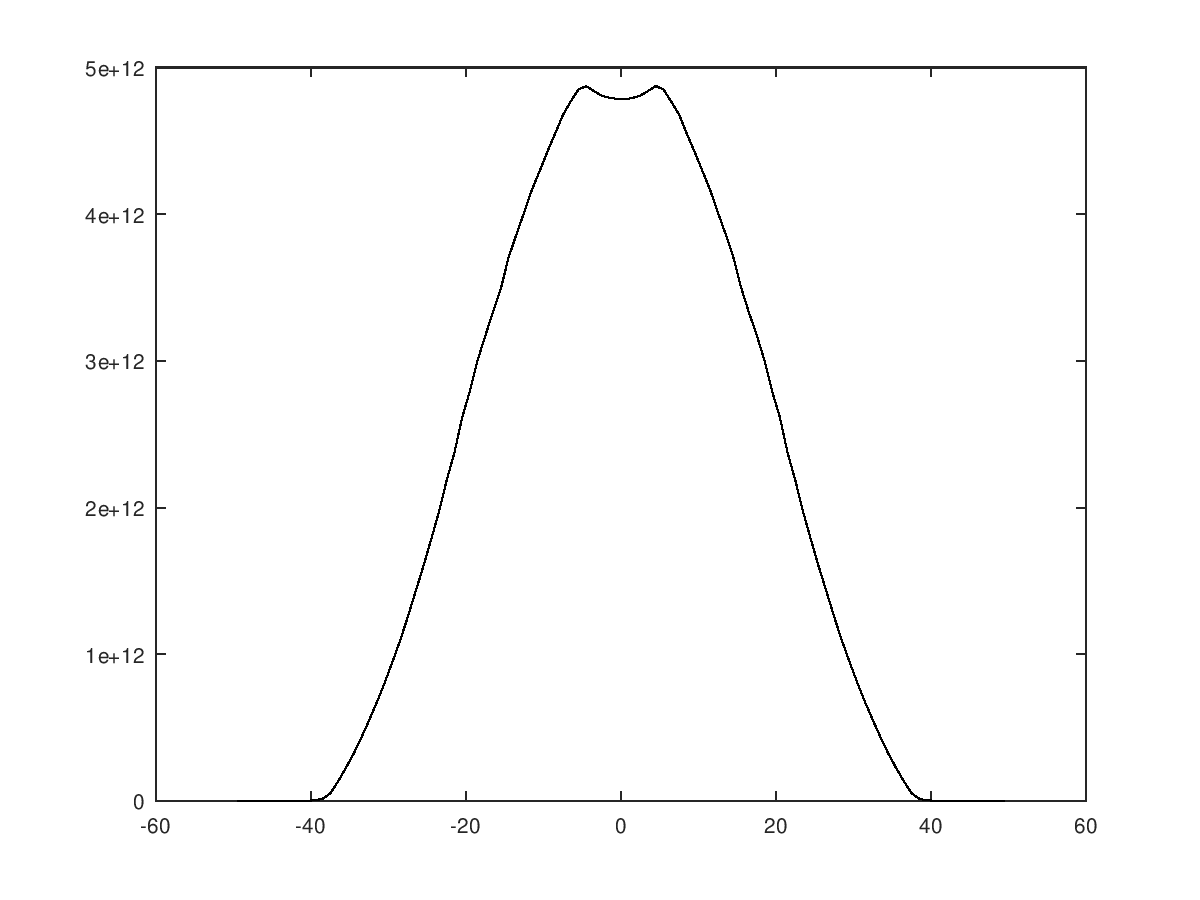
\includegraphics[width=\textwidth]{Figuras/ch2_intens.png}
    \caption{Perfil radial de intensidad}\label{fig:ch2_intensidad}
  \end{subcaptionblock}
  \begin{subcaptionblock}{.4\textwidth}
    \centering
    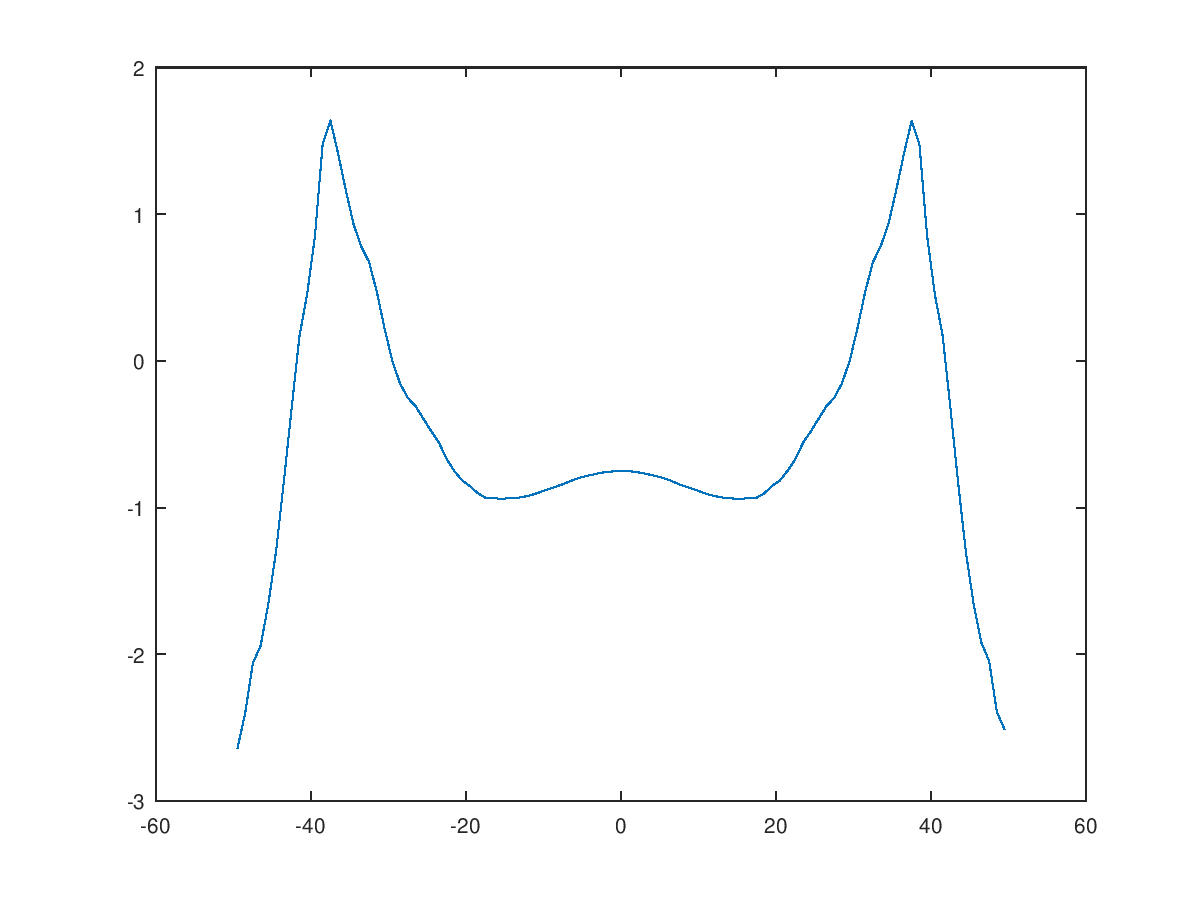
\includegraphics[width=\textwidth]{Figuras/ch2_fase.png}
    \caption{Perfil radial de fase}\label{fig:ch2_fase}
  \end{subcaptionblock}
  \caption{Curvas de intensidad y fase obtenidas mediante el código Dagon. El eje de abscisas representa la dimensión radial (en \unit{µm}), y los ejes de ordenadas la intensidad (en \unit{W/cm^{2}}) y la fase (en \unit{rad}) del haz amplificado.} 
  \label{fig:2.1}
\end{figure}

El capítulo \S\ref{cap:4} está dedicado a la presentación, análisis y recopilación de los resultados obtenidos. Frecuentemente, ejecutar un experimento en óptica y fotónica de sistemas láser puede ser un camino realmente complejo y costoso, motivando el desarrollo de métodos matemáticos capaces de simular con suficiente precisión el comportamiento observado durante el experimento. Por ello, otro objetivo básico de este proyecto consiste en caracterizar los principales parámetros que determinan las características ópticas de la luz láser buscada, permitiendo optimizar futuros trabajos e investigaciones experimentales.

Fundamentalmente, la modificación de propiedades del plasma, como la distribución espacial de electrones e iones a través de la columna, las regiones fronterizas entre las distintas especies; o la modificación de las propiedades del armónico inyectado, como la energía y duración del pulso, y la incorporación de un momento angular orbital (\acrshort{oam}) en dicho armónico, permiten realizar este estudio de manera sistemática, apareciendo representados mediante parámetros libres dentro del esquema computacional descrito en la sección \ref{sec:3.2}.

Sin embargo, la cantidad de factores y etapas que participan en la amplificación de la semilla de rayos X blandos durante interacción con el plasma dificulta su estudio. En este sentido, este proyecto está integrado dentro de una línea de investigación más grande, nutrido de las observaciones y los resultados de anteriores estudiantes, como Alba Guiomar Verdejo y Marina Ruiz Izu, cuyas pequeñas aportaciones ayudan, en su conjunto, a continuar expandiendo y mejorar la comprensión del fenómeno.

Finalmente, la inyección de armónicos de alto orden con momento angular orbital ha sido un objeto extenso de estudio, propiedad interesante de cara a sus aplicaciones científica y tecnológicas. Por este motivo, la parte final está dedicada a presentar brevemente la introducción en la distribución espacial-fasorial del armónico un nuevo parámetro, representado por un índice angular $l=25$ en el haz de Laguerre-Gauss, como el explicado durante la sección \ref{sec:1.1.2}, que permita analizar los efectos del \acrshort{oam} en los perfiles radiales estudiados anteriormente, cuando la semilla no transportaba este momento angular, es decir, con un índice angular $l=0$.

\begin{figure}[htbp]
  \centering
  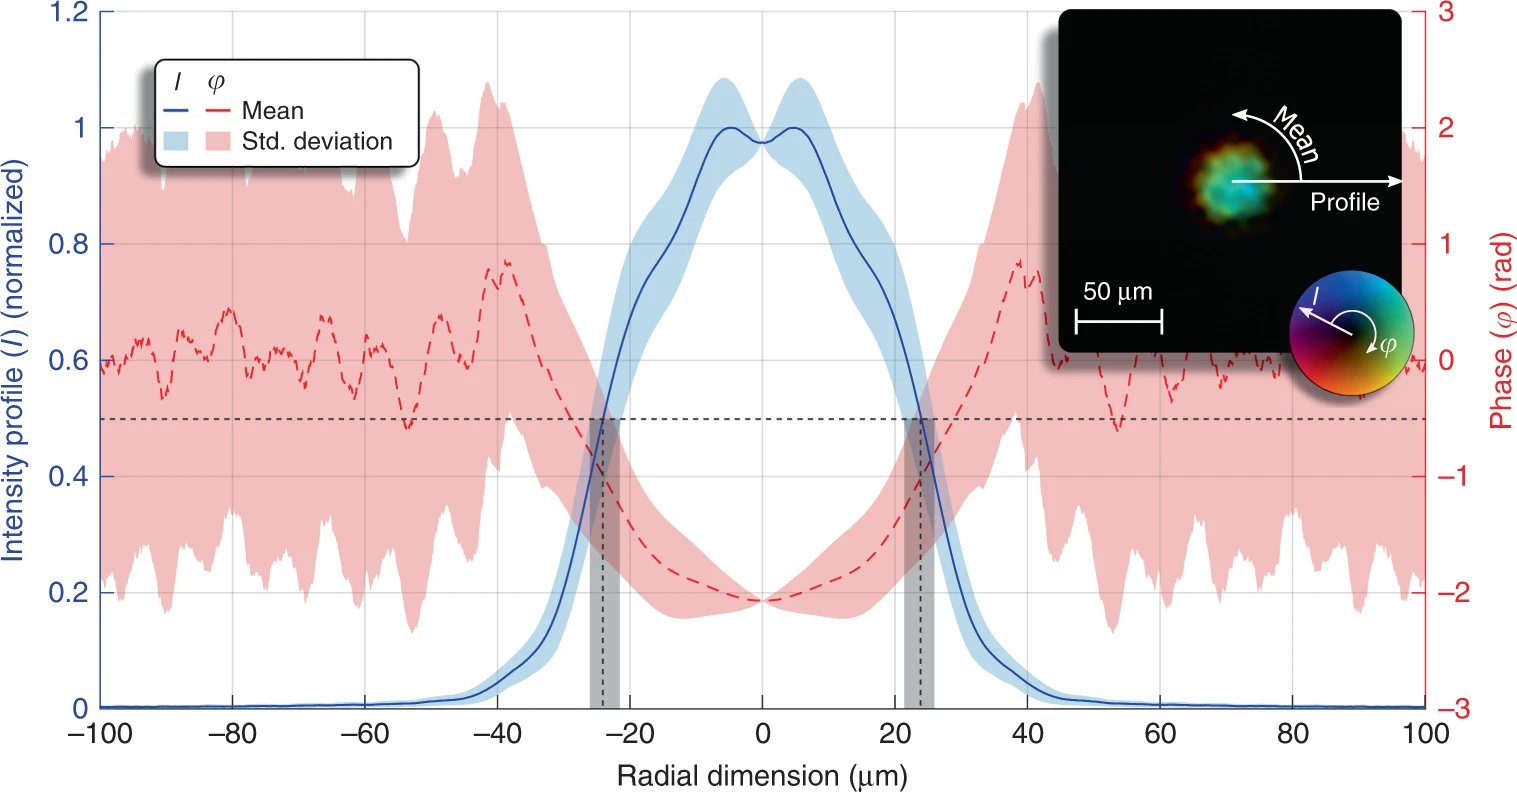
\includegraphics[width=0.9\textwidth]{Figuras/ch2_curvas_lab.png}
  \caption{Reconstrucción del campo de intensidad-fase obtenido a la salida del amplificador láser-plasma. \autocite{Tuitje2020}}
  \label{fig:2.2}
\end{figure}



